\documentclass[12pt]{../SOP4_alpha}\usepackage[]{graphicx}\usepackage[]{color}
% maxwidth is the original width if it is less than linewidth
% otherwise use linewidth (to make sure the graphics do not exceed the margin)
\makeatletter
\def\maxwidth{ %
  \ifdim\Gin@nat@width>\linewidth
    \linewidth
  \else
    \Gin@nat@width
  \fi
}
\makeatother

\definecolor{fgcolor}{rgb}{0.345, 0.345, 0.345}
\makeatletter
\@ifundefined{AddToHook}{}{\AddToHook{package/xcolor/after}{\definecolor{fgcolor}{rgb}{0.345, 0.345, 0.345}}}
\makeatother
\newcommand{\hlnum}[1]{\textcolor[rgb]{0.686,0.059,0.569}{#1}}%
\newcommand{\hlstr}[1]{\textcolor[rgb]{0.192,0.494,0.8}{#1}}%
\newcommand{\hlcom}[1]{\textcolor[rgb]{0.678,0.584,0.686}{\textit{#1}}}%
\newcommand{\hlopt}[1]{\textcolor[rgb]{0,0,0}{#1}}%
\newcommand{\hlstd}[1]{\textcolor[rgb]{0.345,0.345,0.345}{#1}}%
\newcommand{\hlkwa}[1]{\textcolor[rgb]{0.161,0.373,0.58}{\textbf{#1}}}%
\newcommand{\hlkwb}[1]{\textcolor[rgb]{0.69,0.353,0.396}{#1}}%
\newcommand{\hlkwc}[1]{\textcolor[rgb]{0.333,0.667,0.333}{#1}}%
\newcommand{\hlkwd}[1]{\textcolor[rgb]{0.737,0.353,0.396}{\textbf{#1}}}%
\let\hlipl\hlkwb

\usepackage{framed}
\makeatletter
\newenvironment{kframe}{%
 \def\at@end@of@kframe{}%
 \ifinner\ifhmode%
  \def\at@end@of@kframe{\end{minipage}}%
  \begin{minipage}{\columnwidth}%
 \fi\fi%
 \def\FrameCommand##1{\hskip\@totalleftmargin \hskip-\fboxsep
 \colorbox{shadecolor}{##1}\hskip-\fboxsep
     % There is no \\@totalrightmargin, so:
     \hskip-\linewidth \hskip-\@totalleftmargin \hskip\columnwidth}%
 \MakeFramed {\advance\hsize-\width
   \@totalleftmargin\z@ \linewidth\hsize
   \@setminipage}}%
 {\par\unskip\endMakeFramed%
 \at@end@of@kframe}
\makeatother

\definecolor{shadecolor}{rgb}{.97, .97, .97}
\definecolor{messagecolor}{rgb}{0, 0, 0}
\definecolor{warningcolor}{rgb}{1, 0, 1}
\definecolor{errorcolor}{rgb}{1, 0, 0}
\makeatletter
\@ifundefined{AddToHook}{}{\AddToHook{package/xcolor/after}{
\definecolor{shadecolor}{rgb}{.97, .97, .97}
\definecolor{messagecolor}{rgb}{0, 0, 0}
\definecolor{warningcolor}{rgb}{1, 0, 1}
\definecolor{errorcolor}{rgb}{1, 0, 0}
}}
\makeatother
\newenvironment{knitrout}{}{} % an empty environment to be redefined in TeX

\usepackage{alltt}
\usepackage[english]{babel}

\title{Hazardous Materials Handling}
\date{2/24/2018}
\author{EA30-Fall 2015, Virginia Paschal}
\approved{Los Huertos}
\ReviseDate{\today}
\SOPno{02 v0.2}
\IfFileExists{upquote.sty}{\usepackage{upquote}}{}
\begin{document}

\maketitle

\section{Scope and Application}

\NP This SOP covers the safe use, disposal, and spill treatment of hazardous material.

\NP This document applies to staff, students, and researchers who use acid, base, explosive, caustic and poisonous materials.  

\NP This document does not explicitly cover radioactive materials. 

\tableofcontents

\newpage

\section{Definitions}

\begin{description}

  \item[Corrosive Chemicals] Corrosive chemicals include strong acids and bases, dehydrating agents, nonmetal chlorides and halogens. These chemicals are health hazards and present problems in handling and storage. Purchase corrosives in containers with a protective plastic coating, if available.  Store corrosives under the hood, or low shelving or in storage cabinets. Gas cylinders (including lecture sized) should not be stored in the same cabinet with corrosive liquid, because of possible cylinder/valve damage.  Properly segregate hazardous materials to prevent fire, explosion or toxic gas release. For example, segregate acids from bases and oxidizing acids from organic acids. Also, separate nitric acid from other acids. 

\item[Flammable Liquids] Flammable and combustible liquids are chemicals in a liquid state that can easily burn. They are classified, or grouped, as either flammable or combustible by their flashpoints. Flammable liquids will catch on fire and burn easily at normal working temperatures. Combustible liquids have the ability to burn at temperatures that are usually above working temperatures.

\item[Caustic Chemicals] Include a range of chemicals, e.g. ammonium hydroxide, Potassium hydroxide, sodium hydroxide, that are able to burn or corrode organic tissue by chemical action.

\item[Safety Data Sheet (SDS)] Each chemical we use will have a Safety Data Sheet (SDS) describing the hazards associated with the data sheet, and how the material should be handled. These sheets will be on the counter next to east entrance to the room, in the PPE shelves near the entrance of SGM 133.

\end{description}

\section{Health and Safety}

\subsection{Protect Gear}

\NP It is necessary to wear protective gear, such as: close-toed shoes, gloves, goggles when using hazardous equipment.

\subsection{Signage}

\NP Laboratory areas that have special or unusual hazards should be posted with warning signs. Standard signs and symbols have been established for a number of special situations, such as: biological hazards (Figure~\ref{fig:biohzard}) and fire hazards (Figure~\ref{fig:hazard_sign}.


\begin{figure}
  \centering
  \includegraphics[width=0.7\textwidth]{biohazard}
  \caption{he biohazard symbol was developed in 1966 by Charles Baldwin, an environmental-health engineer working for the Dow Chemical Company on the containment products. Generally used as a warning, so that those potentially exposed to the substances will know to take precautions.}
  \label{fig:biohzard}
\end{figure}
\NP Other signs should be posted to show locations of safety showers, eyewash stations, which are located on the right and left sides of the lab, exits, and the fire extinguisher located near the front entrance. Extinguishers should be labeled for the type of fire for which they are intended. Waste containers should be labeled for the type of waste that can be safely deposited. Label all waste containers with the contents, manufacturer's name, appropriate warnings, and hazard class to prevent accidental use and to preserve any specimen or products. 

\subsection{Spill Kit} 

\NP There is a green spill kit mounted on the wall next to the PPE shelves, near the entrance to SGM133. This kit is capable of treat contained spills.

\subsection{Mindfulness in the Laboratory}

Be cautious whilst handling the chemicals; being mindful includes the following characteristics: 

\begin{enumerate}
  \item Reduce distractions in your mind;
  \item Be present in your surroundings;
  \item Reflect on the potential hazards (e.g. carefully evaluate each material using SDS forms and hazard symbology (Figure~\ref{fig:hazard_sign}).
\end{enumerate}

\begin{figure}
  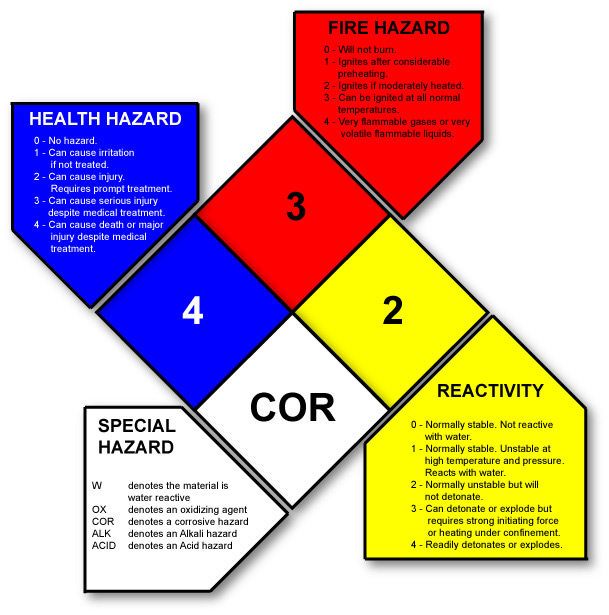
\includegraphics[width=1.0\textwidth]{Hazard_sign}
  \label{fig:hazard_sign}
  \caption{Reflect each of the categories of hazards and how you might respond to each in different ways.}
\end{figure}

\subsection{Hazardous Chemical Handling}

\section{Personnel \& Training Responsibilities}

\NP Proper training entails identifying job-specific hazards and making sure students attend safety training appropriate for their work. 

\NP Each student/researcher must have a proper understanding of materials used and the possible dangers of each material, i.e. to become familiar with the SDS information for every chemical they handle.

\NP Chemical Safety Officer. Every year, one person will be assigned to the job as Chemical Safety Manager. This person will work to maintain laboratory safety by updating SOPs, training all researchers, and ensuring safe laboratory conditions.

\NP Specifically, the Chemical Safety Officer 

\begin{itemize}
  \item ensures all students, technicians, and researchers are trained re-informed and re-assessed about Lab safety periodically throughout their work in the laboratory;
  \item promotes a culture of safety so that all researchers have the same or similar understanding of Lab Safety;
  \item ensures researchers who are performing anything more than basic tasks have a more in depth and specific training for what they are doing. For example, a student whose job it is to operate a piece of machinery should first properly understand how to do so.

\end{itemize}

\subsection*{Training}

\NP All researcher using this SOP should be trained for the following SOPs:

\begin{itemize}
  \item SOP1 Laboratory Safety
\end{itemize}

\section{Required Materials}

\NP Access to SOP and Training Documentation binder

\section{Estimated Time}

\NP Following these guidelines is a key part of the laboratory experience and work, thus be sure to allocate time to read and prepare all laboratory work with attention to safety.

\NP Training requires approximately 20 minutes.


\section{Procedures}

\subsection*{Preparation Before Handling Hazardous Chemicals}

\NP Handling Glassware: Check condition of glassware. Only glass in condition should be used. Discard or send for repair glass that is broken, chipped, starred, or badly scratched. Clean glassware before sending it for repair. 

\NP When picking up broken glass use proper hand protection.

\subsection*{Handling and Transportation of Chemicals}

\NP Many lab accidents occur due to carrying chemicals from one place to another or transferring chemicals from one container to another. 

\NP Because chemicals used in the lab are often corrosive, flammable, or toxic and thus, have the potential for injury, it is good practice to assume that all chemicals are potentially hazardous. 

\NP Wear appropriate Personal Protective Equipment (PPE). Minimum PPE includes safety glasses, lab coat, long pants, and closed-toe shoes.

\NP Large bottles of chemicals should be carried on a cart. If there is not a cart, the bottles should be carried one at a time. The bottle should be carried with two hands, one around the neck of the bottle and one underneath the bottle. Do not hook a finger through the ring on top of the bottle because it will dangle while being transported. Never attempt to pick up a bottle by the cap. A bottle transporter is the safest way to transport. 

\NP When transporting bottles within the lab, a wheeled cart may be used. Do not place bottle near the edge of the cart. The bottles should not be touching each other or other glassware either. Be cautious of rolling carts over door sills or other obstructions.

\NP When transporting outdoors, two people must be present to prevent the cart from tipping over uneven surfaces and changes in elevation.

\NP Incompatible chemicals should not be carried on the same cart. 

\NP Special padded or rubber bottle carriers, carts, or pails should be used to prevent breaking from accidental hitting against walls or floor. 

\NP Individuals transporting chemicals must ensure containers are properly labeled and be informed of what to do in case of a spill or release. 

\NP Hazardous chemicals must be attended at all times while being transported.

\NP If transporting via elevator, Freight-only elevators should be used, if possible, to avoid exposure of chemicals to persons on passenger elevators. If no freight elevators are available, use unoccupied passenger elevators.  

\NP Unstable, explosive, or unusually hazardous materials due to size or toxicity should not be moved. 

\NP Large quantities of concentrated mineral acids should be kept in storage rooms, in cabinets for corrosive substances, or in chemical transfer rooms. Bottles of concentrated acids from the aforementioned areas should be transported in an approved acid bottle carrier. 

\NP Organic solvents should be stored in special flammable storage areas. These solvents can be transported from storage areas in special rubber carriers, as organic solvents prevent fire and inhalation hazards. 

\subsection*{Chemical Storage}

\NP Every chemical should be returned to its storage location after use. 

\NP Solvents, acids, bases, reactives, oxidizers, and toxins should be stored separately.

\NP Separation refers to physical separation of containers and isolation of potential spills and releases to prevent chemical reactions. Separate cabinets or isolated areas within a central storage should be used for storage of incompatibles. Look at compatibility restrictions on cabinets under fumehoods. 

\NP Hazardous chemicals should never be stored on the floor. Containers should be stored in low shelves or in cabinets. The shelves should have a lip on the forward edge to prevent containers from falling off. Shelves should be securely fastened to a wall or floor. Shelves should not be overloaded.

\NP Use a compatible container for storing chemicals or wastes. Metal containers are often unsuitable for corrosive wastes and halogenated solvents, even if the solvents were originally shipped in metal containers. In these instances, plastic carboys or lined metal containers may be more suitable. 

\NP Containers storing chemical waste should be checked weekly for any sign of chemical leakage.

\NP Containers of all types should be free of rust and deformation. 

\NP Caps and covers for containers should remain securely on containers when not in immediate use.

\NP NFPA (National Fire Protection Association) labeling should appear on cabinets and room doors at approximately waist level or lower in order to see the labels in dense smoke conditions.

\NP All containers used for storage should be labeled in compliance with Hazard Communications regulations and NFPA and the college's fire codes. At a minimum, all containers must be labeled with content and general hazard.

\NP Flammable liquids greater than 1 liter should be kept in metal safety cans. Never disable the spring-loaded closure. Always keep flame-arrestor screen in place; replace if punctured or damaged. 

\NP Flammable liquids should not be stored in the lab in amounts greater than the limits for flammable liquid storage given in SOPs. 

\NP Metal drums used for storage and dispensing of flammable chemicals should be properly grounded. Ground cables should be available and used.

\NP Chemicals should stored as close as possible to the point of use to maximize efficiency and minimize transport. Chemical storage should be limited to areas in which the particular chemical is used. Storage locations must be identified on an emergency floor plan posted in each work area.

\NP Small quantities of chemical may be held at individual work stations if it is to be promptly used in a test and does not compromise organic vapor levels or procedures for spill control and fire safety. These containers must be properly labeled.

\NP Only limited quantities of chemicals and solvents should be stored in the lab. Large drums or multiple bottles of chemicals should be stored in a central chemical storage area.

\NP Out-of-date chemicals should be disposed of on a periodic basis to reduce hazard potential and minimize inventory tracking and updating.

\subsection*{Chemical Spill Treatment}

\NP Safety First

\begin{description}
\item[Isolate Spill Area] 
\item[Notify proper authorties] In our cases, calling campus safety is appropriate because they will rely messaage to the appropriate agency, usually the Claremont Fire Department.
\item[Wear adequate protection] PPE includes eye protection, hand protection, and respirtory protection. 
\end{description}

\NP Identify Spill. Determine if it's a acid, caustic, solvent, or other. 

\NP Select Spill Control Agent:

\begin{itemize}
  \item Spill-X-A for acids;
  \item Spill-X-C for caustics; and
  \item Spill-X-S for solvents.
\end{itemize}

\NP Treat Spill 

\begin{enumerate}
  \item Encircle and cover spill with agent;
  \item mix agent with spill using provided scraper; 
\begin{itemize}
  \item For acids and bases will be a neutralization reaction and leave a paste like substance. 
  \item For solvents, agent adsorption is indicated by the disappearance of free liquid.
\end{itemize} 
\end{enumerate}
  
\NP Restore Area
\begin{enumerate} 
  \item Test representative samples of spill residue for final PH. Add more agent if necessary. 
  \item Use SPILL-X-S to solidify any remaining liquid. Final spill residue should be dry and powdery.
  \item Record spill type, treatment e.g. ``neutralized acid/base,ph=$\rule{1cm}{0.15mm}$", ``adsorbed solvent:name",and disposition i.e. recommended disposal method onto the labels of provided bags. 
  \item After treatment reaction cools, use provided scraper and pan to pick up residue and place into labeled bag.
  \item Rinse and decontaminate utensils and spill area.
\end{enumerate}

\subsection*{Chemical Waste Disposal}

\NP Chemical waste containers: Containers used to the accumulation of hazardous waste must be in good condition, free of leaks and compatible with the waste being stored in them. The waste container should be capped, only opened when adding waste. Hazardous waste must not be placed in unwashed containers that previously held incompatible materials.  A storage container holding a hazardous waste that is incompatible with waste or materials stored nearby in other containers must be separated from the other materials  sto or protected by a wall, partition, or other secondary containment device. 

\NP Labeling containers: Before chemicals can be disposed of, a waste tag is required. It should be filled out by the waste generator and attached to each container. Manifest is also required. 

\NP Waste minimization: Avoid buying and using large quantities when not necessary. 

\NP Flammable organic solvents: Flammable organics can often be reused for fuel unless they are extremely toxic or give off toxic products of combustion. Halogenated solvents, acutely toxic flammable, acids, bases, heavy metals, oxidizers, and pesticides should be collected in separate containers. The compounds most suitable for recovery include: Acetone, 2-Butanol, Butly alcohol, Butyl alcohol, Cyclohexane, Diethyl ether, Ethyl acetate, Ethyl alcohol, Heptane, Hexane, Methyl alcohol, Methyl cellosolve, Pentane, Petroleum ether, 2-Propanol, Sec-butyl alcohol, Tert-butyl alcohol, Tetrahydrofuran, Xylene. Do not combine any of the previous listed flammable organic solvents with any other chemicals. 
Disposal of chemicals down sink or sanitary sewer system:
Very few chemical wastes are acceptable for disposable down the sink or sanitary sewer system. Small-scale research activities (100 mL or less) of certain types of water-soluble, nontoxic, and nonflammable chemicals may be poured if they have been approved by the Chemical Safety Director. 

\NP Waste Disposal Procedures: Collect each chemical waste in a separate screw-top container. Do not mix wastes. Use the smallest container size to match the amount of chemical waste generated. The container the chemical was originally shipped in is an ideal waste collection container, if the size is suitable. Waste containers should be securely capped. Each container must be labeled as to chemical content. For mixtures, give approximate percentages of each chemical compound. Completely fill chemical waste collection containers. Shock-sensitive and water-reactive compounds and lecture bottles require special handling. These materials should be packed separately from other chemicals. Chemicals that have potential to react with other chemicals should not be packed in the same box. Determine the packing hazard class for each chemical waste, prioritizing reactivity over toxicity. Segregate the wastes according to hazard class and pack them into different cardboard boxes for each hazard class. Place dividers and shock absorbing materials (newspapers, vermiculite) between the containers. 

\NP The label for the chemical waste is called a packing manifest. A manifest must be attached to each box. A manifest should include: lab information and waste information. The generator should check the information on the manifest, sign their name, and attach it to the corresponding box. 

\NP Attach one copy to the box and keep a copy for lab records. Specify where the waste is to be picked up. 

\NP Chemical substitution: Whenever possible, substitute nonhazardous, biodegradable chemicals for hazardous chemicals. Use of these chemicals will reduce the volume of hazardous waste generated. 
Chemical Safety-Labeling, and Hazardous Chemicals

\NP Labeling. All containers should be dated and labeled with the chemical components and hazards. It is recommended that the user’s name also appear on the label. Labels on incoming containers are not to be removed or defaced. Dating is especially important in the case of compounds which have a specified shelf life, such as those that will form peroxides. Identifying unknown materials for disposal is extremely costly. Chemical names must be spelled out on labels. Chemical formulas, acronyms, and abbreviations are not acceptable as the only identification of the contents of a container. Laboratory samples, including field specimens and newly synthesized compounds, must be identified as accurately as possible. In cases where the container is unable to be labeled, steps should be taken to ensure the contents can be identified.

\NP Examples of  warning signs:


\subsection*{Lessons Learned}

\NP Unfortunately, history is rife with instances of laboratory safety breakdowns.  However, by analyzing the causes of laboratory accidents we can identify patterns that consistently lead to both positive and negative safety results.  Listed below are common laboratory accidents and how to prevent them.

\NP Cuts: Prevent cuts in lab by disposing of all sharp metal and glass properly.  Inspect glassware for cracks prior to use.  Use extreme care around glass in lab. (Dartmouth)

\NP Burns: Minimize fire hazard by using hot plates or water baths instead of open flames.  Tie up loose hair and wear snug clothing, avoiding synthetic materials when possible.  Always use a fume hood when working with volatile organic compounds (Dartmouth).

\NP Chemical spills: Anyone who is working with a hazardous chemical needs to read the chemicals’ safety data sheet before beginning work.  Additionally, personal protective equipment should always be worn, unused chemical containers capped, and engineering controls such as fume hoods used when necessary.  You should never work alone in the laboratory.  More important than anything is awareness.  Always think through all actions and be careful (Pomona).

\NP Mercury Poisoning: ... as well as Mercury Spills: http://www.pomona.edu/sites/default/files/emergency-instructions.pdf)

\NP Explosions: Due to the unique nature of each potentially explosive chemical reaction in the laboratory, it is important to develop written protocols for the handling of explosive chemicals and process, as well as to familiarize all lab workers with the protocols.  Use of fume hoods, avoidance of carrying out experiments in closed containers, and use of PPE can all reduce the potential for an explosive event.  (Texas Tech)

\NP Chemical Inhalation: Never breathe deeply from a chemical mixture.  In addition to working in a fume hood, it is advisable to use equipment that can monitor the amount of gas coming off of an experiment. (Dartmouth)


\section{References}

\NP APHA, AWWA. WEF. (2012) Standard Methods for examination of water and wastewater. 22nd American Public Health Association (Eds.). Washington. 1360 pp. (2014).
\end{document}
